\clearpage
\item \subquestionpoints{5} \textbf{Coding problem.}
We will now tune the hyperparameter $\tau$.
In \texttt{src/p05c\_tau.py}, find the MSE value of your model on the 
validation set for each of the values of $\tau$ specified in the code. For each
$\tau$, plot your model's predictions on the validation set in the format
described in part (b). Report the value of $\tau$ which achieves the lowest MSE
on the \texttt{valid} split, and finally report the MSE on the \texttt{test}
split using this $\tau$-value.

\ifnum\solutions=1 {
  \begin{answer}
The value of $\tau$ which achieves the lowest MSE on the valid split is 0.05, and the corresponding MSE on the test split is 0.0170.\\
Figures of the predictions on the valid set are on the next page.
\begin{figure}[htb]
    \begin{subfigure}{0.5\linewidth}
        \centering
        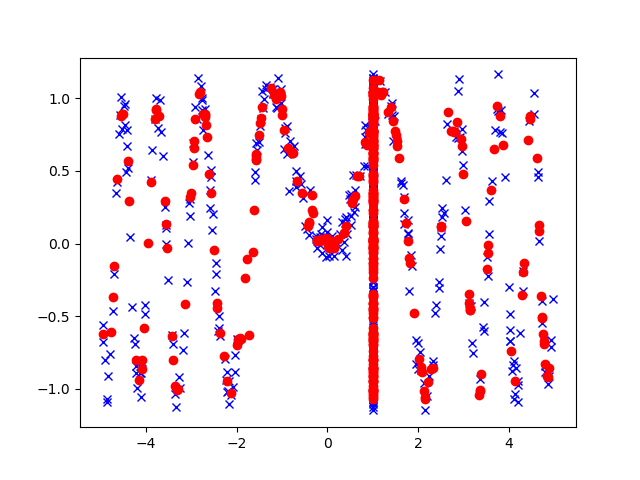
\includegraphics[width=\linewidth]{tex/tau_0.03.png}
        \subcaption*{tau=0.03}
    \end{subfigure}
    \begin{subfigure}{0.5\linewidth}
        \centering
        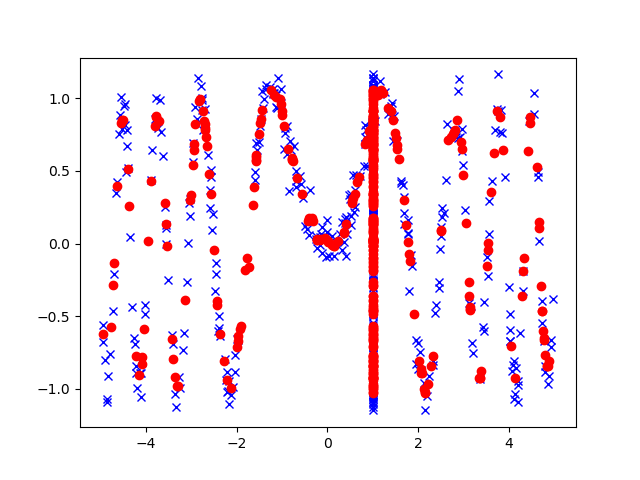
\includegraphics[width=\linewidth]{tex/tau_0.05.png}
        \subcaption*{tau=0.05}
    \end{subfigure}
    \begin{subfigure}{0.5\linewidth}
        \centering
        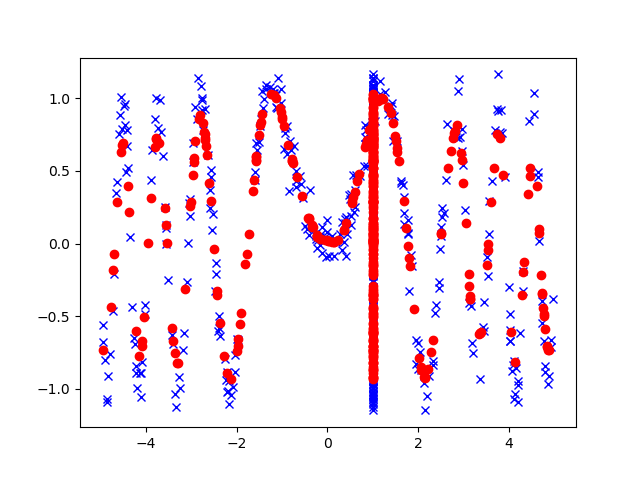
\includegraphics[width=\linewidth]{tex/tau_0.1.png}
        \subcaption*{tau=0.1}
    \end{subfigure}
    \begin{subfigure}{0.5\linewidth}
        \centering
        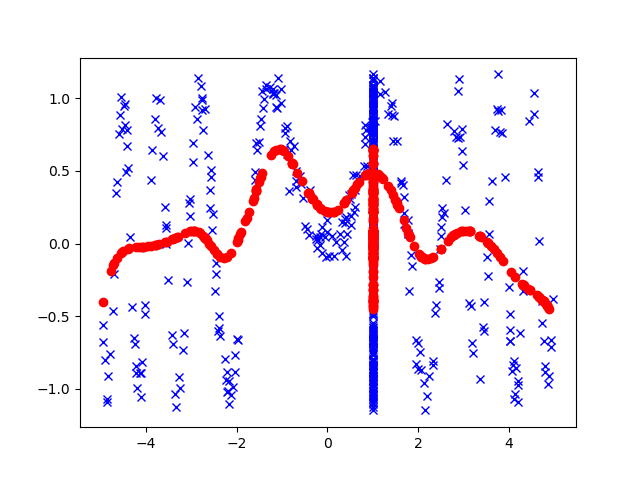
\includegraphics[width=\linewidth]{tex/tau_0.5.png}
        \subcaption*{tau=0.5}
    \end{subfigure}
    
    \begin{subfigure}{0.5\linewidth}
        \centering
        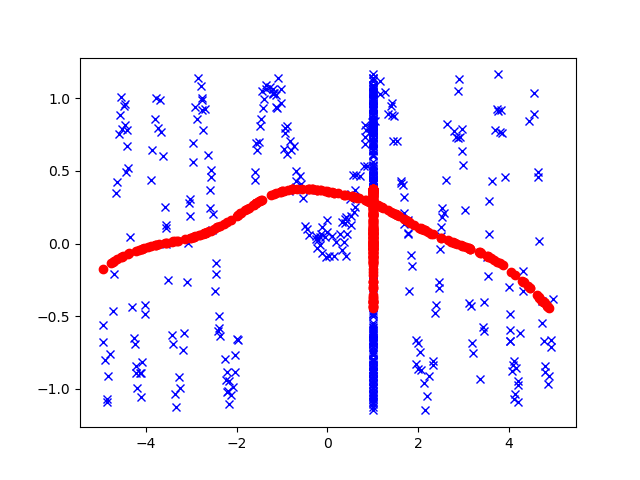
\includegraphics[width=\linewidth]{tex/tau_1.0.png}
        \subcaption*{tau=1.0}
    \end{subfigure}
    \begin{subfigure}{0.5\linewidth}
        \centering
        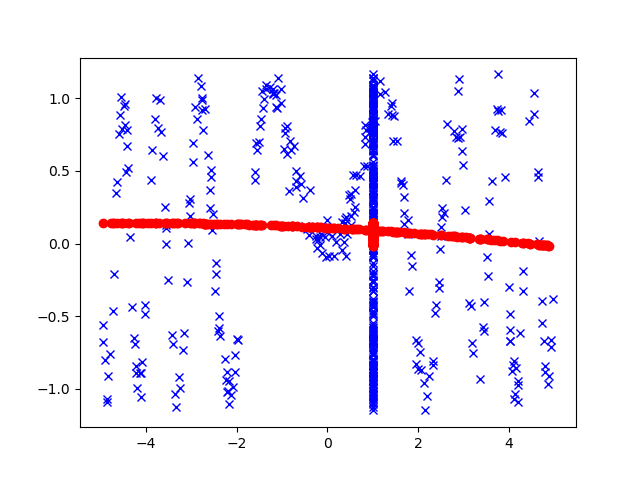
\includegraphics[width=\linewidth]{tex/tau_10.0.png}
        \subcaption*{tau=10.0}
    \end{subfigure}
\end{figure}
\end{answer}

} \fi
